The UCLA HEDP package is separated into several sub-packages (folders within the package) that group similar routines. The logic of these groupings, and a brief explanation of the contents of each sub-package, is provided in the following sections.

\begin{figure}[h]
\centering
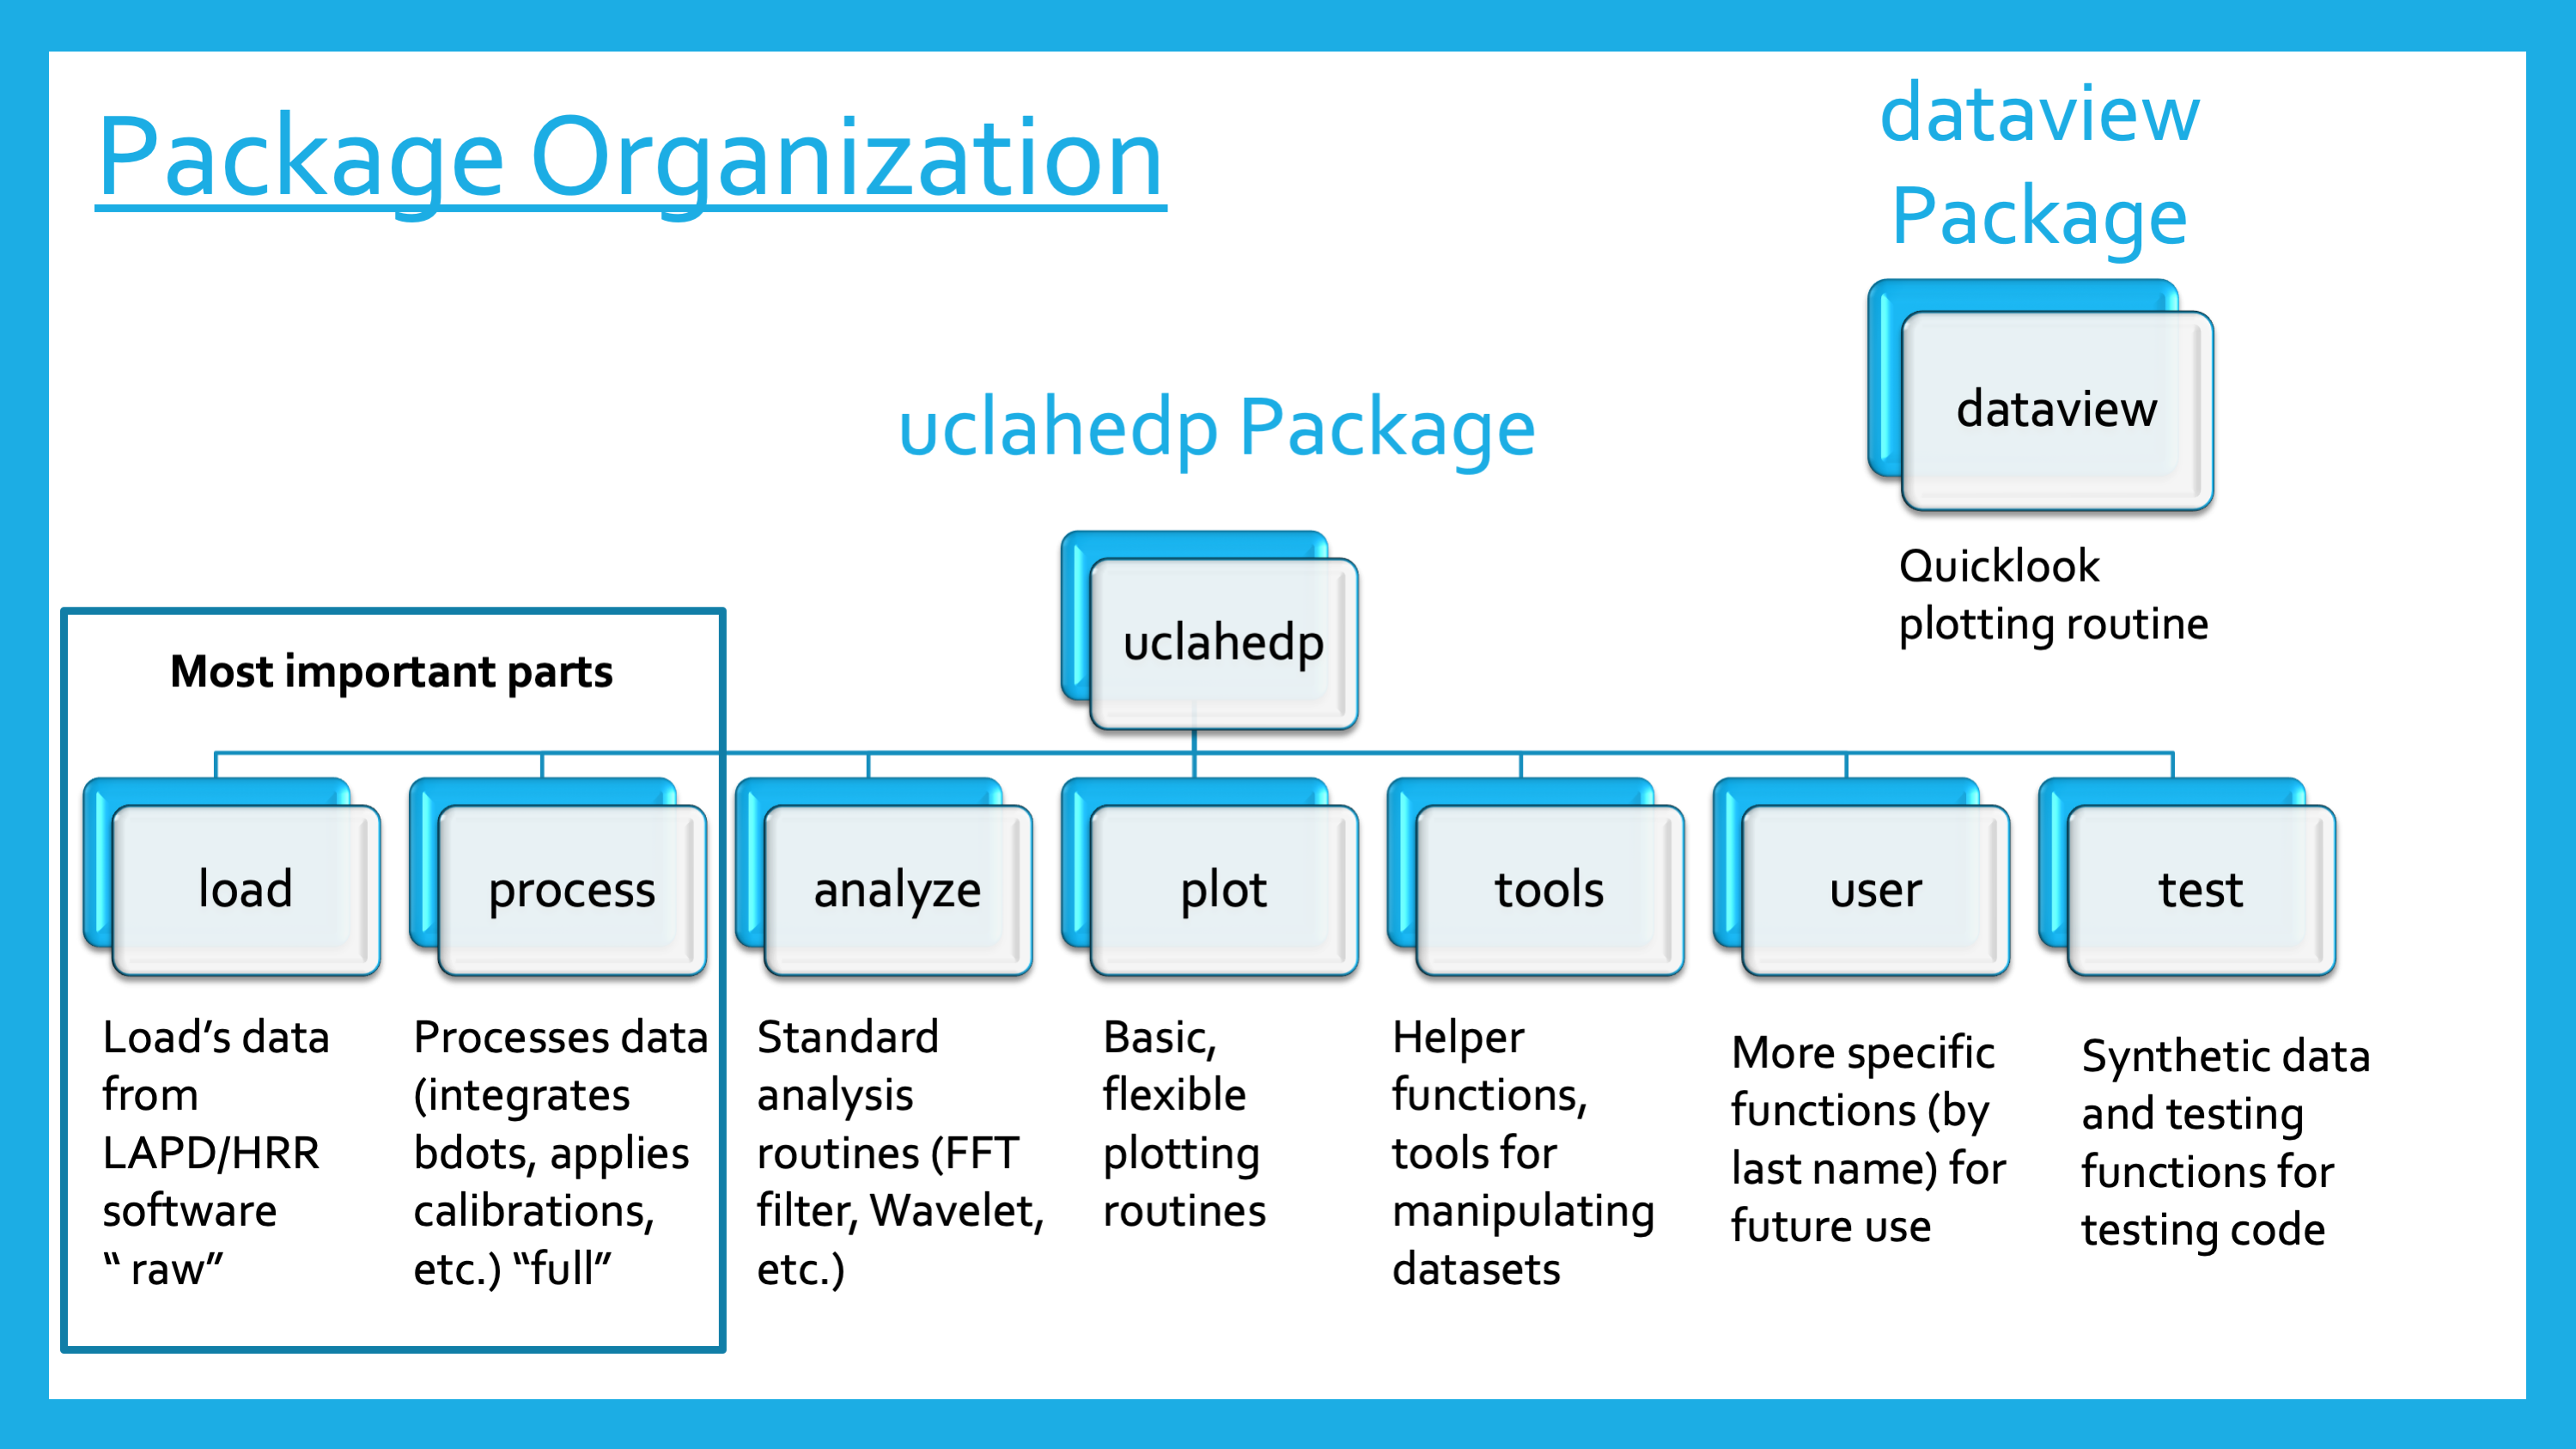
\includegraphics[width=\textwidth]{package_struct}
\caption[Package Structure]
{\label{package_struct} An organizational diagram showing the relationships between the different parts of the package.}
\end{figure}


\subsection{\loc{tools}}

The \loc{tools} package contains a variety of miscellaneous functions, many of which are used widely throughout other routines.
\subsubsection{\loc{csv.py}}

The primary purpose of \loc{csv.py} is to process a directory of comma-separated value (CSV) files in a file directory containing metadata about an experiment (see Sec.~\ref{csv_format}).  A list of CSV files in a directory is created using \loc{csv.getCSVList} and then those files are read into a python OrderedDictionary object by \loc{csv.opencsv}. This package is commonly accessed from other routines through the function \loc{csv.getAllAttrs}, which returns the metadata from across all files that pertains to a particular probe and run number. Functions \loc{csv.getProbeList} and \loc{csv.getRunList} provide lists of all valid probes and runs from an experiment, which are useful when creating loops to process data.


\subsubsection{\loc{dataset.py}}

This file contains a function that tests whether an HDF group conforms with the CDF (as described in Sec.~\ref{cdf}), which is \loc{dataset.validDataset}. Another helper function \loc{createDataset} can be used to create new datasets from a group of arrays.

The remainder of this file contains functions that were intended to perform operations over large datasets in an efficient way. The function \loc{dataset.chunked\_array\_op} was intended to provide an easy way to perform operations like thinning and averaging large datasets without forcing the user to manually chunk the data. However, this scheme turned out to be too time intensive because data operations are applied one-by-one. At this time, the most efficient way to process a large dataset is still to write a custom program that performs all operations in a single pass through the file (a process which is difficult to generalize).

\subsubsection{\loc{hdf.py}}

This file contains programs for interfacing with HDF files. In particular, \loc{hdf.writeAttrs}, \loc{hdf.readAttrs}, and \loc{hdf.copyAttrs} are the preferred way to interact with attributes because they correctly translate strings to unicode and handle the (value,unit) format used in the CDF. This file also contains the \loc{hdf.hdfPath} object which is provides a convenient way to pass both a filename and a HDF group path as one object. This was created with the idea of eventually supporting HDF files with multiple CDF objects within them (as separate groups).

\subsubsection{\loc{math.py}}

This file contains mathematical functions used throughout the package. In practice most routines necessary are available in \loc{numpy} or other packages, so the only function here is a discrete curl algorithm.

\subsubsection{\loc{pos.py}}

This file contains routines for creating grids for volumetric measurements. The functions are generally called through the high-level function \loc{pos.grid}, which takes a list of positions (along with some required attributes) and outputs a list of axes as and an array for placing shots into a grid. Two steps are necessary for this process: the creation of axes and the placement of points on those axes. Two methods exist for carrying out these operations, dubbed "strict" and "fuzzy" gridding. Which of these methods is applied is controlled by keywords.

Under strict axes, axes are created \textit{a priori} based on metadata in the attributes dictionary, while under fuzzy axes axes are inferred from the provided position array. Similarly, under strict gridding shots are assigned to positions in the grid based on an \textit{a priori} assumption about the movement of the probe (and metadata), whereas under fuzzy gridding positions are discritized (to within the grid precision) and placed at the grid cell that most closely matches the probes actual location. These methods can be mixed, eg. strict axes can be used with fuzzy gridding. 

In general, fuzzy axes and gridding are more desirable. These ensure that the true location of the probes is used (a probe may not actually move to a location if it is physically unable to do so, which is not reflected in strict gridding). Fuzzy gridding also easily supports complicated probe paths and could easily be upgraded to support non-cartesian grids. Strict axes and gridding should be viewed as a backup for datasets on which fuzzy gridding fails for some reason.

\todo{Modification of these routines to support grids in polar coordinates should be a relatively high priority in future in order to support "fan" grid patterns on radial probe drives like those on the LAPD.}


\subsubsection{\loc{util.py}}

This file contains several convenience functions, the most widely used of which is the \loc{util.timeRemaining} object which is used to create progress timers for various operations throughout the package.

\subsection{\loc{load}}

The \loc{load} subpackage provides routines for transforming data from several sources into the standard CDF format. Once data is in this format, it can be processed by other routines in the package without regard to its origin.

Load routines also take a csv directory and merge the relevant attributes (based on the selected probe and run) with the dataset. This metadata is then attached to the HDF file, so changing the metadata necessitates re-processing the data from the beginning starting with the load command. This choice was made intentionally to ensure that consistent metadata is used throughout the processing of a dataset.

\subsubsection{\loc{lapd.py}}

These programs load data from HDF files output by the LAPD DAQ system using the \loc{bapsflib} package. The routine can currently import position information from three probe drives: the XY drive, the XYZ drive, and the XY drive (6K Compumotor). 

\todo{Originally only the 6K Compumotor was supported by \loc{bapsflib}, and so the other drives were handled manually. Support for other drives has now been added to \loc{bapsflib}, so these routines could be updated to use that functionality.}

\subsubsection{\loc{hrr.py}}

These programs load data from HDF files output by the Phoenix Terminal's High Repetition Rate experiment software. 

\subsubsection{\loc{imgdir.py}}

This program loads a directory of images, commonly used to import frames from a camera. Images are loaded in an order determined by their filenames using a natural sorting algorithm.


\subsubsection{\loc{ascii.py}}

This program loads data from an ASCII file, intended for creating CDF objects out of simulation output or output from instruments like oscilloscopes. 

\todo{This program may not be finished, but would be a useful tool. An additional desirable feature would be the ability to load whole directories of ASCII files and combine them intelligently into one CDF.}


\subsection{\loc{process}}

The \loc{process} subpackage is the core of the UCLA HEDP package, containing routines that transform raw data into processed data ready for analysis. Each file described below processes data for a particular diagnostic or instrument. The example script \loc{process.process.py} shows how all of these routines (along with those throughout the package) can be used to turn raw datasets and metadata files into processed output files.

\subsubsection{\loc{bdot.py}}

The primary function in this file is \loc{bdot.bdotRawToFull} which processes raw magnetic flux probe measurements into measurements of the vector magnetic field. Several of the keywords in this function merit some explanation

\begin{itemize}
\item \loc{replace\_badshots} If this keyword is set, shots marked as bad by the tdiode routine will be copied over by the nearest good shot.

\item \loc{offset\_range} gives the range (in indices) over which the voltage offset of the signal will be calculated. This should done at a time when the real signal is nominally zero. 

\item \loc{offset\_rel\_t0} allows the user to set values in the previous variable as being relative to to the laser firing. A common configuration is for the start of the offset range to be fixed at zero, but the end to be set to be just before the laser pulse. In this case the user may set \loc{offset\_range} = (0, -50) while \loc{offset\_rel\_t0} = (False, True). 
\end{itemize}

This file also contains two functions \loc{bdot.fullToCurrent} and \loc{fbdot.ullToBmag} which take a fully processed bdot signal and calculate either the current (using the curl and neglecting the displacement current in Ampere's law) or the magnitude of B. 

The file also contains the \loc{bdot.calibrateProbe} function which performs fits to calibration data recorded in a CSV file by a network analyzer. This program assumes a standard Helmholtz coil configuration is used to calibrate the probe. 

\todo{The current \loc{bdot.calibrateProbe} function can only handle CSV files, while the network analyzer used at UCLA for this purpose outputs \loc{.dat} files. Reading these files directly should be possible, and adding that functionality to this function would be very helpful.}

\subsubsection{\loc{tdiode.py}}

This program takes in data from a timing diode (typically a photodiode positioned in the leak of a laser mirror that shows the laser pulse) and determines the index corresponding to the rise of the pulse (corresponding to t0). The program also identifies bad shots (no laser) by comparing the maximum of the pulse to the noise level. 


\subsubsection{\loc{langmuir.py}}

This file contains several programs for processing Langmuir probe measurements. \loc{langmuir.isatRawToFull} processes ion saturation current measurements and is relatively straight forward. \loc{langmuir.vsweepLangmuirRawToFull} processes swept Langmuir probe measurements and is considerably more complicated. The swept Langmuir probe routine makes use of several subroutines

\begin{itemize}

\item \loc{langmuir.find\_sweeps} takes a time array and a voltage trace of the ramp voltage and identifies the time ranges corresponding to each ramp. By default the swept Langmuir analysis routine will attempt to fit ever ramp (although many at lower densities may fail). 

\item \loc{langmuir.vsweep\_fit} takes a Langmuir IV curve (voltage and current traces) and fits the electron saturation and transition regions with a linear fit and an exponential fit respectively. The program attempts to intelligently determine the boundaries for these regions, but they may also be adjusted by the user. This function is designed to recognize failed fits, which are commonly caused when a probe moves into a region of lower density. These failed fits are intended to cause errors which results in the value \loc{fail\_val} being output in the parameters so these datapoints can be easily ignored in analysis.

\todo{Some rudimentary error analysis is in place for this function: in principle it should be possible to transform the covariences from the curve fits into error bars on the output quantities like density and electron temperature. In practice propagating the the errors from both fits through the formulas is non-trivial, but this would be a great project to finish in the future.}

\end{itemize}


\subsubsection{\loc{interferometer.py}}

This file contains a simple routine for computing the phase shift measured by an interferometer from a hetrodyne interferometer given the signal and the reference signal. 

\todo{The full calculation of the density from the phase shift has not yet been implemented.}

\subsubsection{\loc{imgseq.py}}

This file contains a function that transforms a CDF file created from an image directory corresponding to a sequence of images and creates appropriate physically meaningful axes for it. Attributes can be set in the metadata to change the scale of the pixels in physical units, set an origin, and create a time vector. 

\subsubsection{\loc{scope.py}}
This program is a dummy processing routine that does nothing to the data other than apply a timing diode correction. The intended use-case is for quick analysis during an experiment of instruments that are not otherwise handled by the UCLA HEDP package.

\subsubsection{\loc{process.py}}
This script is an example/template script for running all of the analysis programs in the UCLA HEDP package. The program \loc{process.process} takes runs the full sequence of analysis steps on a probe for a particular run. A raw file is created using the appropriate load function, then the appropriate final processing routine is applied.

\loc{process.processMany} runs this program in a loop over a set of runs and probes provided by the user. Combinations of runs and probes that do not apply are ignored. This allows the user to set up a large list of runs and probes (potentially an entire experiment) to run unattended.

\todo{This file should really live in the examples folder, since it's really just an example of a processing script.}





\subsection{\loc{analyze}}

The \loc{analyze} subpackage contains useful routines for data analysis. 

\subsubsection{\loc{filter.py}}
This file contains several frequency filtering tools that can be used for either temporal or spatial frequency filtering. \loc{filter.fftFilter} is a Fourier-filter than provides a bandpass (or band-block) filter on a 1D trace. \loc{filter.lowpassFilter2D} is a lowpass filter intended for spatially filtering 2D planes prior to calculating the curl in order to calculate the current.



\subsubsection{\loc{polarization.py}}

This file contains functions for analyzing the polarization of a signal based on a vector time trace either using a polarization decomposition algorithm or by creating a hodograph.

\subsubsection{\loc{spectral.spectrogram.py}}

This function implements a moving-window Fourier transform algorithm to generate a spectrogram. 

\subsubsection{\loc{thomson.thomson\_scattering.py}}

This file contains a number of routines for the prediction of Thomson scattering spectra. \loc{thomson\_scattering.spectrum} calculates the spectral density function in a variety of regimes given a description of the ion and electron distributions (assuming Maxwellians). \loc{thomson\_scattering.signal\_estimate} estimates the total number of scattered photons for use in estimating the signal-to-noise ration for a given configuration.

This program was developed prior to the implementation of \loc{diagnostics.thomson} in PlasmaPy: the implementation there is better vetted and you are encouraged to use that instead.


\subsection{\loc{user}}

Any user of the package is invited to add a folder to this section which holds code they have written that either uses the package or complements it.


\subsection{\loc{dataview}\label{dataview}}

The \loc{dataview} program is technically a separate program from UCLA HEDP (housed in a different repository) so that it can be installed without as many requirements. \loc{dataview} can visualize any CDF object. One of the benefits of using a consistent data format is that \loc{dataview} can therefore be used to look at data saved at any point during the analysis pipeline.